\section{Trading Strategy}

%----------------------------------------------------
\subsection{Beta-neutral positions on every $(i,j)\in\mathcal B$}
Since we are interested in the individual effect of an article $i\in\D$ in each of the affected firms $j\in\F^i$, we work with the set
$
\mathcal{B}:=\3{(i,j) \mid i\in \D ~\wedge~j\in \F^i }
$, where $\abs{\mathcal{B}}=3410>\abs{\D}=2613$. 
We then fit a market model to each unique pair $(i,j)\in \mathcal{B}$
on a lookback window of 100 days with a buffer of 10 days before the effective treatment date $\tilde d_0^i$. %$\mathcal{M}^i\subset \tilde{\mathfrak{d}}$ before the effective treatment day,%
%------------------- START FOOTNOTE-------------------
%\footnote{$\mathcal M_i$ is a window of $w_m=100$ days formed with a buffer of $w_b=10$ days  before the effective treatment date $\tilde d_0^i$. Formally, it is defined as   
%$
%\mathcal{M}^i := 
%\{
%d\in \tilde{\mathfrak{d}}
%\mid 
%\mathbb{I}^{-1}_{\tilde{\mathfrak{d}}} 
%(
%\mathbb{I}_{\tilde{\mathfrak{d}}} (\tilde{d}_0^i) - {w}_b - {w}_m 
%)
%\leq d \leq 
%\mathbb{I}^{-1}_{\tilde{\mathfrak{d}}} 
%(
%\mathbb{I}_{\tilde{\mathfrak{d}}} (\tilde{d}_0^i) - {w}_b 
%)
%\}
%,
%$
%where $\mathbb{I}_{\tilde{\mathfrak d}}$ maps an element $d\in\tilde{\mathfrak d}$ to its position in $\tilde{\mathfrak d}$ and $\mathbb{I}^{-1}_{\tilde{\mathfrak d}}$ does the inverse mapping. 
%}
%%
%----------------------------------------------------
%
$$
r_{d}^{j} = \alpha^{(i,j)} + \beta^{(i,j)} r_{d}^M + \epsilon_{ d}^{(i,j)} 
%\qquad  
%\forall d \in \mathcal{M}^i
,
$$
where 
$r_{d}^{j}$ denotes the return of firm $j$ at trading day $d$ in excess of the risk-free asset, which we take to be the daily euro short-term rate (\texttt{\euro STR}),
and 
$r_{d}^M$ denotes the excess return of the market (IBEX-35).  
%----------------------------------------------------
These returns are obtained from adjusted close prices, which correct the price evolution for corporate actions such as dividends, stock splits, and new stock issuance.
%\footnote{
%The adjusted close price ensures that the returns reflect the true economic gains or losses for an investor holding the stock. 
%%
%Formally, the return of firm $j$ between two trading days $d_1, d_2\in \tilde{\mathfrak{d}}$ is computed as:
%$
%r_{d_1:d_2}^{j} = 
%(
%p_{d_2}^{j,\text{adj}} - p_{d_1}^{j,\text{adj}}
%)/(
%p_{d_1}^{j,\text{adj}}
%)
%$
%where $p_{d}^{j,\text{adj}}$ is the adjusted close price of firm $j$ at trading day $d$.
%}
%----------------------------------------------------
%
%\mx 
%----------------------------------------------------
The notation overload in the regression coefficients $(\alpha^{(i,j)},\beta^{(i,j)})$ emphasizes the fact that $\alpha$ and $\beta$ are specific to each pair $(i,j)\in\mathcal B$ since the market model is computed for each firm $j\in\F_{\t{IBEX-35}}$ on a lookback window of time 
	%$\mathcal{M}^i$, 
	which is particular to each article $i\in\D$.
%----------------------------------------------------

\mx 
The reason why we fit a market model to each $(i,j)\in\mathcal B$ is to then apply a market-neutral strategy as in 
\cite{chan2003stock} % Chan (2003)
and 
\cite{jiang2021pervasive}. % Jiang et al. (2021).
This is an investment approach designed to minimize or eliminate exposure to overall market movements, isolating the performance of a specific firm. 
% 
In particular, we employ a beta-neutral strategy by buying one unit of firm $j$'s stock and shorting $\beta^{(i,j)}$ units of the market index (i.e.: an ETF replicating the IBEX-35). 
%----------------------------------------------------
This hedged position harvests the idiosyncratic returns from the market model and it only makes sense when firm $j$'s returns are expected to outperform or underperform the market.\footnote{
For expected underperformance of firm $j$, reverse the beta-neutral positions: 
sell one unit of firm $j$ and buy $\beta^{(i,j)}$ units of the market index. However, note that this will be handled later by a Trading Rule $(TR)$.
\sx 
}
The position delivers abnormal returns $AR^{(i,j)}_{d}$ at some trading day $d\geq \tilde{d}_0^i$ given by
\begin{align*}
r_{d}^j -  \beta^{(i,j)} r_{d}^M = \alpha^{(i,j)} + \epsilon_{d}^{(i,j)} =: AR^{(i,j)}_{d}
.
\end{align*}
%----------------------------------------------------
The position is taken at the effective treatment date $\tilde d_0^i$ and is maintained over a holding window %$\mathcal H^i \subset \tilde{\mathfrak{d}}$ 
	consisting of $L\in\mathbb{N}$ trading days after $\tilde d_0^i$, where $L$ is set to 4 trading days.
%\footnote{The holding period of the position is defined as 
%$
%\mathcal H^i:=
%\{
%d \in \tilde{\mathfrak{d}}
%\mid 
%\tilde{d}_0^i
%\leq d \leq 
%\mathbb{I}^{-1}_{\tilde{\mathfrak{d}}}(\mathbb{I}_{\tilde{\mathfrak{d}}}(\tilde d_0^i)+L)
%\}
%$}
%----------------------------------------------------
The justification for this choice of $L$ results from the maximization of the Sharpe Ratio of the portfolio in the train and validation samples for both KMeans and LLM-based clustering.\footnote{ 
The choice of $L$ is justified in detail in \ref{sec:A2}, and the sensitivity of the trading strategy's out-of-sample performance to different values of $L$ is examined in Section \ref{sec:6} (\qquote{Robustness Checks}).
}
%----------------------------------------------------
Finally, we compute the Sharpe Ratio of each position $SR^{(i,j)}$, which we will subsequently employ to optimize cluster selection.
%----------------------------------------------------
%After having held the beta-neutral position over the holding period $\mathcal H^i$, we obtain a time series of abnormal returns $\{AR_{d}^{(i,j)}\}_{d\in\mathcal H^i}$ from where we can obtain the usual performance metrics. First, the average daily log returns are obtained as
%$$
%\mu^{(i,j)} = \frac{1}{{{L}}+1} 
%\sum_{d\in \mathcal H^i}
%\ln\4{1+AR_d^{(i,j)}}
%~,
%$$
%Then, the standard deviation is given by
%$$
%\sigma^{(i,j)}
%=
%\sqrt{
%\frac{1}{{{L}}}
%\sum_{d\in \mathcal H^i}
%[
%\ln(1+AR_d^{(i,j)}) - \mu^{(i,j)}
%]
%^2}
%~.
%$$
%
%\mx 
%And finally, the annualized Sharpe Ratio can be obtained by scaling the daily Sharpe Ratio by the square root of ${252}$, which are the typical number of trading days in a year according to the Spanish calendar. 
%$$
%SR^{(i,j)} =
%\sqrt{252}~
%\frac{
%\mu^{(i,j)}
%}{
%\sigma^{(i,j)}
%}
%~.
%$$
%----------------------------------------------------

%%%%%%%%%%%%%%%%%%%%%%%%%%%%%%%%%%%%%%%%%%%%%%%%%%%%%
\subsection{Optimal Cluster Selection}
%%%%%%%%%%%%%%%%%%%%%%%%%%%%%%%%%%%%%%%%%%%%%%%%%%%%%

After taking beta-neutral positions on each pair $(i,j)\in\mathcal B$ and holding them over $L$ days, 
%some window $\mathcal H^i$, 
we can obtain a measure of how profitable the positions are on average for articles that belong to the same cluster.
% $g\in\mathcal G$. 
For this purpose, let $\mathcal{B}_g$ denote the set of all article-firm pairs such that the article belongs to some cluster $g\in\mathcal G$. 
$$
\mathcal{B}_g:= \{(i,j) \mid (i,j)\in\mathcal{B} ~\wedge~ i \in \D_g \}
.
$$
The average Sharpe Ratio associated to each cluster is
$$
\overline{S R}_g=\frac{1}{\left|\mathcal{B}_g\right|} \sum_{(i,j) \in \mathcal{B}_g} S R^{(i,j)}
,
$$
and it provides a measure of the performance of the beta-neutral positions in each cluster. 
%
%
The distribution of cluster-average Sharpe Ratios across the different clusters is shown in Appendix \cref{fig:cluster-average-SR-by-split}. 


%%%%%%%%%%%%%%%%%%%%%%%%%%%%%%%%%%%%%%%%%%%%%%%%%%%%%
%%%%%%%%%%%%%%%%%   ALGORITHMS   %%%%%%%%%%%%%%%%%%%%
%%%%%%%%%%%%%%%%%%%%%%%%%%%%%%%%%%%%%%%%%%%%%%%%%%%%%
\mx
We then focus on developing two algorithms that optimally leverage the cluster information for our trading strategy. Our approach draws parallels with traditional portfolio sorting methods, where assets are typically arranged into deciles based on specific characteristics, and trading positions are established by going long on top deciles and short on bottom ones. Similarly, our strategy will construct self-financing portfolios based on clusters rather than individual assets: taking long positions in clusters expected to outperform and short positions in those expected to underperform.
%
To identify the optimal clusters for trading, we propose two distinct algorithmic approaches. The first approach, which we term \qquote{greedy}, selects clusters by maximizing the Sharpe Ratio within the validation dataset. The second approach, termed \qquote{stable}, utilizes a broader information set by incorporating both training and validation data, aiming to identify clusters that maintain consistent performance across both splits. In both algorithms, we impose sign restrictions to ensure that our trading positions align with the expected direction of returns.

\subsubsection{Greedy Algorithm}

The greedy selection of clusters is done in the validation sample 
$
\mathcal{B}^{val}:= \{
(i,j)\in\mathcal{B} 
 \mid 
  i \in \D^{val} \}
~,
$
from where we compute the cluster-average $\overline{S R}_g^{val}$ for each $g\in\G$.
%
%----------------------------------------------------
Define $\mathcal G_{SR^+}^{val}:=\{ g\in \mathcal G \mid \overline{SR}_g^{val} >0\}$ and $\mathcal G_{SR^-}^{val}:=\{ g\in \mathcal G \mid \overline{SR}_g^{val} <0\}$ as the sets of clusters with positive and negative Sharpe Ratios in the validation sample. Obviously, we will be interested in taking long positions when reading an article that is clustered in some $g\in \mathcal G_{SR^+}^{val}$, and short positions in clusters $g\in \mathcal G_{SR^+}^{val}$. 
%
%\mx 
%----------------------------------------------------
However, our trading strategy will not trade every cluster $g\in\G$. Instead, it will select the clusters from $\mathcal G_{SR^+}$ and $\mathcal G_{SR^-}$ that lead the to most profitable trades. 
To identify such clusters, we rank them by their average Sharpe Ratio. Define the ranking function $\mathfrak{R}: \mathcal{G} \to \3{1, \ldots, k^*}$ such that
$$
\mathfrak{R}_g^{val}
=
\sum_{h \in \mathcal{G}} 
\mathbf{1}\1{
\overline{S R}_h^{val} \geq \overline{S R}_g^{val} 
}
~,
$$
where $\mathbf{1}(\cdot)$ is the indicator function which equals 1 if the condition inside is true and 0 otherwise.

\mx
%----------------------------------------------------
The number of traded clusters on either side (long and short) will be upper-bounded by some hyperparameter of our choice $\theta \in \mathbb{N}$
%$\theta \in \{2 m \mid m \in \mathbb{N}\}$ 
which we set proportional to the number of clusters. Namely, $\theta =\integer{\rho k}$ for some $\rho\in(0,1)$, which has been set to $\rho=0.5$ to maximize the Sharpe Ratio of the trading strategy in the training and validation samples
\footnote{ The choice of $\theta$ is justified in detail in \ref{sec:A2}. The sensitivity of the trading strategy's out-of-sample performance to different values of $\theta$ is examined in Section \ref{sec:6} (\qquote{Robustness Checks}).}.
%
The actual number of traded clusters will not be exactly $\theta$ as there is a natural bound coming from the cardinalities of $\mathcal G_{SR^+}$ and $\mathcal G_{SR^-}$. Hence, the actual number of long and short-traded clusters will be
$
\theta^+ := \min(\theta, ~|\mathcal G_{SR^+}|)
~\t{and}~
\theta^- := \min(\theta, ~|\mathcal G_{SR^-}|)
.
$
%----------------------------------------------------
The set of traded clusters $\mathcal G_{\theta}$ is defined as
$$
\G_\theta := 
\3{
g \in \mathcal G 
\mid 
1\leq \mathfrak{R}_g^{val} \leq \theta^+
~\vee~ 
k^* -\theta^- < \mathfrak{R}_g^{val} \leq k^*
} 
= 
\G_{\theta}^+ \cup \G_{\theta}^-
~,
$$
where
$
\G_{\theta}^+ := 
\{ g \in\G \mid 
1\leq \mathfrak{R}_g^{val} \leq \theta^+
\}
$
is the set of long-traded clusters,
$
\G_{\theta}^- := 
\{ g \in\G \mid 
k^*-\theta^-
< \mathfrak{R}_g^{val} \leq 
k^*
\}
$
is the set of short-traded clusters 
and, clearly, $\abs{\G_{\theta}}=\theta^+ + \theta^- $.\footnote{
Alternatively, we could trade the same number of clusters in the long and short side by defining a unique 
$
\theta^* := \min\1{\theta, |\mathcal G_{SR^+}|, |\mathcal G_{SR^-}| }
%,
$
such that
$
\G_\theta := 
\3{
g \in \mathcal G 
\mid 
1\leq \mathfrak{R}_g^{val} \leq \theta^*
~\vee~ 
k^*-\theta^* < \mathfrak{R}_g^{val} \leq k^*
} 
$
and 
$\abs{\G_\theta}=2\theta^*$.
}
In Appendix \cref{alg:greedy_selection}, we can find the formal design of this algorithm.

%%%%%%%%%%%%%%%%%%%%%%%%%%%%%%%%%%%%%%%%%%%%%%%%%%%%%
\subsubsection{Stable Algorithm}
%%%%%%%%%%%%%%%%%%%%%%%%%%%%%%%%%%%%%%%%%%%%%%%%%%%%%

In this case, we prioritize the stability of the cluster rankings by ensuring that the traded clusters minimize the rank difference of the cluster-average Sharpe Ratios between the training and validation samples. 
To begin, we compute the rank of each cluster based on the average Sharpe Ratios in both the training and validation samples. This delivers $\{\mathfrak{R}_g^{tr}\}_{g\in\G}$ and $\{\mathfrak{R}_g^{val}\}_{g\in\G}$, which provides a measure of the relative performance of the clusters within each sample.

\mx 
Next, we calculate the absolute difference in ranks between the training and validation samples for each cluster, which allows us to measure the stability of each cluster's performance between the two samples
%
$$
\delta_{g} := | \mathfrak{R}_{g}^{tr} - \mathfrak{R}_{g}^{val} |
~.
$$

Clusters are then sorted based on their rank differences $\delta_{g}$ in descending order. To do this, we can simply compute the ranking of the ranking differences as
$$
\mathfrak{R}(\delta_g) := \sum_{h\in\G} \mbf{1}\1{\delta_g \geq  \delta_h }
.
$$
Next, we select the top $2\theta\in\mathbb{N}$ clusters with the smallest rank differences, indicating the most stable clusters across the training and validation samples. The selected clusters now are
%denoted as $\mathcal{G}_{\theta}$
$$
\mathcal{G}_{\theta} = 
\3{
g\in\G \c 1 \leq \mathfrak{R}(\delta_g) \leq 2\theta 
}
.
$$

Finally, we determine the sets of long and short-traded clusters based on the average Sharpe Ratios in both the training and validation samples. In particular, the set of long-traded clusters ($\mathcal{G}_{\theta}^{+}$) are the ones that have positive average Sharpe Ratios in both, training and validation samples
$$
\mathcal{G}_{\theta}^{+} = \{g \in \mathcal{G}_{\theta} \mid \overline{SR}_{g}^{tr} > 0 ~\wedge~ \overline{SR}_{g}^{val} > 0\}
,
$$
and by symmetry, short-traded clusters ($\mathcal{G}_{\theta}^{-}$) are the ones that have negative average Sharpe Ratios in both, training and validation samples
$$
\mathcal{G}_{\theta}^{-} = \{g \in \mathcal{G}_{\theta} \mid \overline{SR}_{g}^{tr} < 0 ~\wedge~ \overline{SR}_{g}^{val} < 0\}
~.
$$


This approach ensures that we select the most stable clusters for trading, reducing the risk associated with rank variability between the training and validation samples, and ensuring that the direction of the signal is consistent across the two splits. The final output consists of the sets of long-traded and short-traded clusters, which are then used to implement the trading strategy.
%
%
The implementation of the algorithm is methodically presented in Appendix \cref{alg:rank_stability}


%%%%%%%%%%%%%%%%%%%%%%%%%%%%%%%%%%%%%%%%%%%%%%%%%%%%%
%%%%%%%%%%%%%%%%%%   KMEANS   %%%%%%%%%%%%%%%%%%%%%%%
%%%%%%%%%%%%%%%%%%%%%%%%%%%%%%%%%%%%%%%%%%%%%%%%%%%%%
%----------------------------------------------------
\inserthere{tab:KMeans_Clusters_Signal}

\begin{table}[H]
\centering
{\fontsize{11}{12.5}\selectfont
\caption{Mapping of embeddings-based KMeans clusters to Trading Signals}
%\begin{tabular}{|c|L{13cm}|c|c|} 
\begin{tabular}{cL{13cm}cc} 
\hline \Xhline{2\arrayrulewidth}
%\rowcolor{gray!10}
\multicolumn{2}{c}{\textbf{Cluster}} & \textbf{Greedy} & \textbf{Stable} \\ \hline \Xhline{2\arrayrulewidth}
0 & Miscellaneous (Colonial, Acciona, Amadeus, Grifols, Endesa, IAG, Bankinter...) &  \textcolor{darkred}{\textsc{short}} &  \\ \hline
1 & Quarterly \& Semi-Annual Earnings Reports &  \textcolor{darkred}{\textsc{short}} &  \\ \hline
2 & BBVA \& Sabadell: Financial Performance \& Strategic Movements &  \textcolor{darkred}{\textsc{short}} &  \\ \hline
3 & Telef�nica \& Cellnex: Telecommunications Tower Sales \& Market Dynamics &  \textcolor{darkgreen}{\textsc{long}} & \textcolor{darkgreen}{\textsc{long}} \\ \hline
4 & CaixaBank: Mergers and Strategic Moves in the Banking Sector &   &  \\ \hline
5 & Telef�nica, Indra, \& M�sM�vil: Regulatory and Strategic Moves in Telecom &  \textcolor{darkgreen}{\textsc{long}} &  \\ \hline
6 & Siemens Gamesa: Supply Agreements, Profitability Targets in Renewable Energy &  \textcolor{darkred}{\textsc{short}} &  \\ \hline
7 & Cellnex: Strategic Acquisitions and Financial Moves in Telecom Infrastructure &  \textcolor{darkgreen}{\textsc{long}} &  \\ \hline
8 & Acciona, Endesa, Enag�s \& Naturgy: Strategic Moves \& Regulatory Developments in the Energy Sector &  \textcolor{darkgreen}{\textsc{long}} &  \\ \hline
9 & Repsol: Strategic Moves and Challenges in the Energy Sector &  \textcolor{darkgreen}{\textsc{long}} &  \\ \hline
10 & Ferrovial, Acciona: Strategic Expansions and Financial Maneuvers in Infrastructure &  \textcolor{darkred}{\textsc{short}} & \textcolor{darkred}{\textsc{short}} \\ \hline
11 & Solaria: Strategic Moves and Market Challenges in Renewable Energy &  \textcolor{darkgreen}{\textsc{long}} & \textcolor{darkgreen}{\textsc{long}} \\ \hline
12 & Iberdrola: Strategic Collaborations and Renewable Energy Developments &  \textcolor{darkred}{\textsc{short}} &  \\ \hline
13 & IAG: Financial Performance &  \textcolor{darkgreen}{\textsc{long}} &  \\ \hline
14 & Santander \& CaixaBank: Financial Moves and Sustainability Initiatives &  \textcolor{darkred}{\textsc{short}} &  \\ \hline
15 & ACS \& Acciona: Strategic Movements and Infrastructure Projects &  \textcolor{darkred}{\textsc{short}} & \textcolor{darkred}{\textsc{short}} \\ \hline
16 & Telef�nica: Financial Performance and Strategic Moves &  \textcolor{darkgreen}{\textsc{long}} &  \\ \hline
17 & Meli� and Spanish Tourism Sector: Challenges Amidst the Pandemic &  \textcolor{darkred}{\textsc{short}} &  \\ \hline
18 & Takeover Bids for Naturgy and M�sM�vil &  \textcolor{darkred}{\textsc{short}} &  \\ \hline
19 & Naturgy: Financial Performance &  \textcolor{darkred}{\textsc{short}} & \textcolor{darkred}{\textsc{short}} \\ \hline
20 & PharmaMar, Grifols: Regulatory Approvals and Market Moves in the Pharmaceutical Sector &  \textcolor{darkgreen}{\textsc{long}} & \textcolor{darkgreen}{\textsc{long}} \\ \hline
21 & Repsol: Financial Performance &  \textcolor{darkgreen}{\textsc{long}} & \textcolor{darkgreen}{\textsc{long}} \\ \hline
22 & Aena: Financial Performance &  \textcolor{darkgreen}{\textsc{long}} & \textcolor{darkgreen}{\textsc{long}} \\ \hline
23 & Enag�s, Endesa, Iberdrola, Red El�ctrica: Regulatory and Market Challenges in the Energy Sector &  \textcolor{darkred}{\textsc{short}} &  \\ \hline
24 & BBVA, CaixaBank, Banco Sabadell: Layoffs and Restructuring &  \textcolor{darkgreen}{\textsc{long}} & \textcolor{darkgreen}{\textsc{long}} \\ \hline
25 & Inditex, Acerinox: Market Performance and Strategic Developments in the Post-Covid Context &  \textcolor{darkred}{\textsc{short}} & \textcolor{darkred}{\textsc{short}} \\ \hline \Xhline{2\arrayrulewidth}
\end{tabular}
\label{tab:KMeans_Clusters_Signal}
}
\subcaption*{\textit{
{ Note: Mapping of embeddings-based KMeans clusters to their Trading Signal \textsc{(long/short)} for the two proposed cluster-selection algorithms (Greedy and Stable). The Greedy algorithm longs (shorts) clusters that maximize (minimize) the cluster-average-$SR$ in the validation sample subject to a positivity (negativity) constraint, while the Stable algorithm longs (shorts) clusters that minimize the rank difference between the training and validation rankings of the cluster-average-$SR$'s subject to a positivity (negativity) constraint, which is now imposed on both sample splits. In both algorithms, the cardinality of each leg is upper-bounded by a hyperparameter $\theta$. Cluster labels are proposed based on the articles they pool. 
}
}}
\end{table}
%----------------------------------------------------
In Table \ref{tab:KMeans_Clusters_Signal} we show the 26 clusters with their proposed names (based on the articles they pool together as shown in Appendix \cref{tab:KMeans_Articles_3_English}) and the selection of long and short-traded clusters according to each algorithm: \qquote{greedy} and \qquote{stable}. We write ``\textsc{long}'' for those clusters $g\in\G_\theta^+$ and ``\textsc{short}'' for $g\in\G_\theta^-$. 
%
%\mx 
As we can see, trading clusters of news articles based on this procedure is quite risky, as there is a high reliance of the signal on the past performance of a cluster. For example, clusters 21 and 22 are linked to the financial performance of Repsol and Aena, respectively, during the training and validation samples. Evidently, the future performance of these firms can change, but the signal provided by the algorithm will still indicate ``\textsc{long}''. 
%
%\bx 
Additionally, some clusters are heavily built on specific events of the period of time they were constructed upon. For example, cluster 17 pools articles related to the challenges of the tourism industry in Spain in Covid times, and cluster 25 is related to the post-covid developments of Inditex and Acerinox. Thus, a clustering approach based on embeddings is not generalizable over time. As the world evolves, clusters become outdated and require constant recalibration to maintain their relevance and predictive power. Hence, any trading strategy based solely on historical cluster performance is likely to produce misguided trading signals over time 

%%%%%%%%%%%%%%%%%%%%%%%%%%%%%%%%%%%%%%%%%%%%%%%%%%%%%
%%%%%%%%%%%%%%%%%%%%%%%%%%%%%%%%%%%%%%%%%%%%%%%%%%%%%
%%%%%%%%%%%%%%%%%%%%   LLM   %%%%%%%%%%%%%%%%%%%%%%%%
%%%%%%%%%%%%%%%%%%%%%%%%%%%%%%%%%%%%%%%%%%%%%%%%%%%%%
%%%%%%%%%%%%%%%%%%%%%%%%%%%%%%%%%%%%%%%%%%%%%%%%%%%%%
%----------------------------------------------------
\inserthere{tab:LLM_cluster_mapping_extended}

\begin{table}[H]
\caption{Mapping of LLM-based clusters to Trading Signals}
\centering
%{\footnotesize
\begin{tabular}{C{1cm}lcc}
\hline \Xhline{2\arrayrulewidth}
%\rowcolor{gray!10}
 \multicolumn{2}{c}{\textbf{Cluster}} & \textbf{Greedy} & \textbf{Stable} \\ \hline \Xhline{2\arrayrulewidth} 
0 & {(demand, minor, positive)} &  &  \\ \hline
1 & {(demand, minor, negative)} &  & \textcolor{darkred}{\textsc{short}} \\ \hline
2 & {(demand, major, positive)} & \textcolor{darkred}{\textsc{short}} & \textcolor{darkred}{\textsc{short}} \\ \hline
3 & {(demand, major, negative)} & \textcolor{darkgreen}{\textsc{long}} & \textcolor{darkgreen}{\textsc{long}} \\ \hline
\Xhline{2\arrayrulewidth}
4 & {(supply, minor, positive)} & \textcolor{darkgreen}{\textsc{long}} &  \\ \hline
5 & {(supply, minor, negative)} & \textcolor{darkred}{\textsc{short}} &  \\ \hline
6 & {(supply, major, positive)} & \textcolor{darkgreen}{\textsc{long}} &  \\ \hline
7 & {(supply, major, negative)} & \textcolor{darkred}{\textsc{short}} &  \\ \hline
\Xhline{2\arrayrulewidth}
8 & {(financial, minor, positive)} & \textcolor{darkgreen}{\textsc{long}} & \textcolor{darkgreen}{\textsc{long}} \\ \hline
9 & {(financial, minor, negative)} &  & \textcolor{darkred}{\textsc{short}} \\ \hline
10 & {(financial, major, positive)} & \textcolor{darkgreen}{\textsc{long}} &  \\ \hline
11 & {(financial, major, negative)} & \textcolor{darkred}{\textsc{short}} &  \\ \hline
\Xhline{2\arrayrulewidth}
12 & {(technology, minor, positive)} & \textcolor{darkgreen}{\textsc{long}} &  \\ \hline
13 & {(technology, minor, negative)} &  &  \\ \hline
14 & {(technology, major, positive)} & \textcolor{darkred}{\textsc{short}} &  \\ \hline
15 & {(technology, major, negative)} &  &  \\ \hline
\Xhline{2\arrayrulewidth}
16 & {(policy, minor, positive)} & \textcolor{darkred}{\textsc{short}} & \textcolor{darkred}{\textsc{short}} \\ \hline
17 & {(policy, minor, negative)} & \textcolor{darkred}{\textsc{short}} & \textcolor{darkred}{\textsc{short}} \\ \hline
18 & {(policy, major, positive)} & \textcolor{darkred}{\textsc{short}} & \textcolor{darkred}{\textsc{short}} \\ \hline
19 & {(policy, major, negative)} & \textcolor{darkred}{\textsc{short}} & \textcolor{darkred}{\textsc{short}} \\ \hline
\Xhline{2\arrayrulewidth}
\end{tabular}
%}
\vspace{0.5cm}
\subcaption*{\textit{
Note: Mapping of LLM-based clusters to their Trading Signal \textsc{(long/short)} for the two proposed cluster-selection algorithms (Greedy and Stable). The Greedy algorithm longs (shorts) clusters that maximize (minimize) the cluster-average-$SR$ in the validation sample subject to a positivity (negativity) constraint, while the Stable algorithm longs (shorts) clusters that minimize the rank difference between the training and validation rankings of the cluster-average-$SR$'s subject to a positivity (negativity) constraint, which is now imposed on both sample splits. In both algorithms, the cardinality of each leg is upper-bounded by a hyperparameter $\theta$. Each cluster corresponds to a type of news-implied firm-specific shock identified by our LLM according to the function calling schema.
}}
\label{tab:LLM_cluster_mapping_extended}
\end{table}
%----------------------------------------------------
%\mx 
%\hspace{0.5cm}
In contrast, our LLM-based clustering methodology offers significant advantages by focusing on the fundamental nature of economic shocks rather than historical patterns. This approach provides more robust and generalizable signals that are less susceptible to temporal changes in market conditions. Moreover, unlike the black box nature of vector embeddings, our methodology offers transparency and interpretability in signal generation. This is evident in how the \textit{Greedy} algorithm's cluster selection closely aligns with the direction of economic shocks: negative shocks typically correspond to price decreases and positive shocks to increases. 

Looking at \cref{tab:LLM_cluster_mapping_extended}, we observe that both algorithms consistently short articles classified as policy shocks, regardless of direction, while going long on cluster 8, which contains approximately one-third of news articles (those categorized as undergoing financial minor and positive shocks). This consistent shorting of policy shocks likely reflects markets' general aversion to policy uncertainty, as policy changes --even positive ones-- often create implementation uncertainty and take time for market participants to fully price in. Interestingly, both algorithms also exhibit seemingly counter-intuitive behavior by going long on negative major demand shocks and short on positive major demand shocks. This pattern might suggest a ``mean reversion'' expectation in the algorithms, where major demand shocks are viewed as temporary deviations that will eventually correct: negative shocks present buying opportunities, while positive shocks signal potential overvaluation.

%%%%%%%%%%%%%%%%%%%%%%%%%%%%%%%%%%%%%%%%%%%%%%%%%%%%%
\subsection{Trading Rule \& Portfolio Construction}
%%%%%%%%%%%%%%%%%%%%%%%%%%%%%%%%%%%%%%%%%%%%%%%%%%%%%
For a given selection of clusters $\G_{\theta}^+$ and $\G_{\theta}^-$, we launch trades and hold them for $L=4$ trading days.
%$L\in\mathbb{N}$ trading days over a window $\mathcal H^i$.
%
Formally, the trading rule
% $TR_{{{L}},\theta}\angl{(i,j),d}$ 
 for a pair $(i,j)\in\mathcal{B}$ at trading day ${d}\in\tilde{\mathfrak d}$ is 
%
%----------------------------------------------------
\begin{align*}
TR_{{{L}},\theta}\angl{(i,j),{d}} := \mycases{rllllll}{
+1
&\IF 
&
[
(i,j)\in\mathcal{B}_g
~\wedge~
g \in \G_{\theta}^+
]
~\wedge~
%{d}\in \mathcal H^i
d \in (\tilde d_0^i, \tilde d_0^i + L]
\\
0
&\IF
&
[
(i,j)\in\mathcal{B}_g
~\wedge~
g \not\in \G_\theta ~
]
~\vee~
%{d} \not\in \mathcal H^i
d \not\in (\tilde d_0^i, \tilde d_0^i + L]
\\
-1
&\IF 
&
[
(i,j)\in\mathcal{B}_g
~\wedge~
g \in \G_{\theta}^-
]
~\wedge~
%{d} \in \mathcal H^i
d \in (\tilde d_0^i, \tilde d_0^i + L]
}
~.
\end{align*}
%----------------------------------------------------

In this context, a portfolio is a collection of positions taken in a firm's stocks according to $TR_{{{L}},\theta}\angl{(i,j),{d}}$. In other words, it is the set of all $\angl{(i,j),{d}}$ for which a trade is executed. 
\begin{align*}
\mathcal P:= 
\3{\angl{(i,j),{d}} 
\c 
(i,j)\in\mathcal{B} 
~\wedge~
{d}\in \tilde{\mathfrak{d}}
~\wedge~
TR_{{{L}},\theta}\angl{(i,j),{d}} \neq 0
}
.
\end{align*}
The set of open positions on a particular day ${d}\in\tilde{\mathfrak d}$ is defined as
$$
\mathcal{P}_{ d}
:=
\3{
(i, j) \in \mathcal{B} 
\c 
T R_{L, \theta}\langle(i, j), {d}\rangle \neq 0 
}
,
$$
and the portfolio is rebalanced every day, so each position $(i, j)\in \mathcal{P}_{d}$ receives a weight that is inversely proportional to the total amount of open positions in that day (i.e. $1/|\mathcal{P}_{d}|$).\footnote{
Note that the cardinality of the set of open positions at day ${d}\in\tilde{\mathfrak d}$, denoted as $|\mathcal{P}_{d}|$, can be computed as the sum of the absolute values of the trading rule over all pairs $(i,j)\in\mathcal B$
 for a given trading day $d\in\tilde{\mathfrak{d}}$.
$$
|\mathcal{P}_{ d}|=\sum_{(i,j)\in\mathcal B}
\abs{
TR_{L, \theta}\angl{(i,j),  d}
}
~.
$$
}
This produces an equally-weighted rolling-portfolio similar to 
\cite{jegadeesh1993returns} % Jegadeesh and Titman (1993)
and 
\cite{chan2003stock}. % Chan (2003)
%
The overlapping returns of the portfolio at $d\in\tilde{\mathfrak{d}}$ can be obtained as an average of the abnormal returns weighted by the trading rule, which determines the direction of each position (long or short), and scaled by the number of open positions in that day,
$$
r_{d}^{\mathcal{P}} 
:= 
\frac{1}{|\mathcal{P}_{d}|}
\sum_{(i, j), \in \mathcal{P}_{d}}
T R_{{{L}}, \theta}\angl{(i,j), {d}} 
\cdot 
AR_{{d}}^{(i,j)}
~.
$$

%%%%%%%%%%%%%%%%%%%%%%%%%%%%%%%%%%%%%%%%%%%%%%%%%%%%%
%%%%%%%%%%%%%%%%%%%%%%%%%%%%%%%%%%%%%%%%%%%%%%%%%%%%%
%%%%%%%%%%%%%%%%%%%%%%%%%%%%%%%%%%%%%%%%%%%%%%%%%%%%%
%%%%%%%%%%%%%%%%%%%%%%%%%%%%%%%%%%%%%%%%%%%%%%%%%%%%%
%Finally, defining the mean portfolio return as
%%----------------------------------------------------
%$
%\mu^{\mathcal{P}}:=
%({1}/{|\tilde{\mathfrak{d}}|})
%\sum_{\tilde{d} \in \tilde{\mathfrak{d}}} \ln (1+r_{\tilde{d}}^{\mathcal{P}})
%$
%and the associated standard deviation:
%$ 
%\sigma^{\mathcal{P}}
%:=
%\sqrt{
%({1}/{|\tilde{\mathfrak{d}}|-1})
%\sum_{\tilde{d} \in \tilde{\mathfrak{d}}}
%[\ln
%(1+r_{\tilde{d}}^{\mathcal{P}}
%)-\mu^{\mathcal{P}}]^2} 
%$
%, we can obtain the annualized Sharpe Ratio of the portfolio as
%$ SR^{\mathcal{P}} :=  \sqrt{252} ~
%{\mu^{\mathcal{P}}}/{\sigma^{\mathcal{P}}} 
%$.
%%----------------------------------------------------
%
%

%--------  Evaluating the Trading Strategy  %-----------

%
%\subsection{Evaluating the Trading Strategy}
%\hspace{0.5cm}The trading strategy is evaluated in the test sample by applying $TR\angl{(i,j),d}$ to all $(i,j)\in\mathcal{B}^{test}$. 
%This delivers the portfolio
%\begin{align*}
%\mathcal{P}^{test}=\3{\angl{(i,j),d} \c (i,j)\in \mathcal{B}^{test} ~\wedge~  TR_{L,\theta}\angl{(i,j),d} \neq 0 }
%,
%\end{align*}
%from where we can compute the portfolio returns 
%$
%r_{d}^{\mathcal{P}^{test}} = 
%({1}/{|\mathcal{P}_{d}^{test}|})
%\sum_{(i, j), \in \mathcal{P}_{d}^{test}}
%T R_{{{L}}, \theta}\angl{(i,j), {d}} 
%\cdot 
%AR_{{d}}^{(i,j)}
%,
%$
%and then obtain $\mu^{\mathcal{P}^{test}}$ and $\sigma^{\mathcal{P}^{test}}$. Finally, we evaluate the \textit{out-of-sample} performance of our trading strategy by looking at the Sharpe Ratio in the test sample
%$
%SR^{\mathcal{P}^{test}} = 
%\sqrt{252}~
%{\mu^{\mathcal{P}^{test}}}/{\sigma^{\mathcal{P}^{test}}}
%.$
%%%%%%%%%%%%%%%%%%%%%%%%%%%%%%%%%%%%%%%%%%%%%%%%%%%%%
%%%%%%%%%%%%%%%%%%%%%%%%%%%%%%%%%%%%%%%%%%%%%%%%%%%%%
%%%%%%%%%%%%%%%%%%%%%%%%%%%%%%%%%%%%%%%%%%%%%%%%%%%%%
%%%%%%%%%%%%%%%%%%%%%%%%%%%%%%%%%%%%%%%%%%%%%%%%%%%%%

In \cref{fig:portfolio_returns_comparison} we plot the cumulative gross returns of trading strategies based on KMeans clustering (Panel A) and LLM clustering (Panel B) across different data splits

%----------------------------------------------------
\inserthere{fig:portfolio_returns_comparison}
\begin{figure}[H]
\caption{Comparison of Cumulative Gross Returns across Clustering Approaches}
\label{fig:portfolio_returns_comparison}

% Panel A: KMeans
\begin{subfigure}{\textwidth}
\caption{Panel A: Cumulative Gross Returns of $\mathcal{P}_{\text{KMeans}}$}
\centering
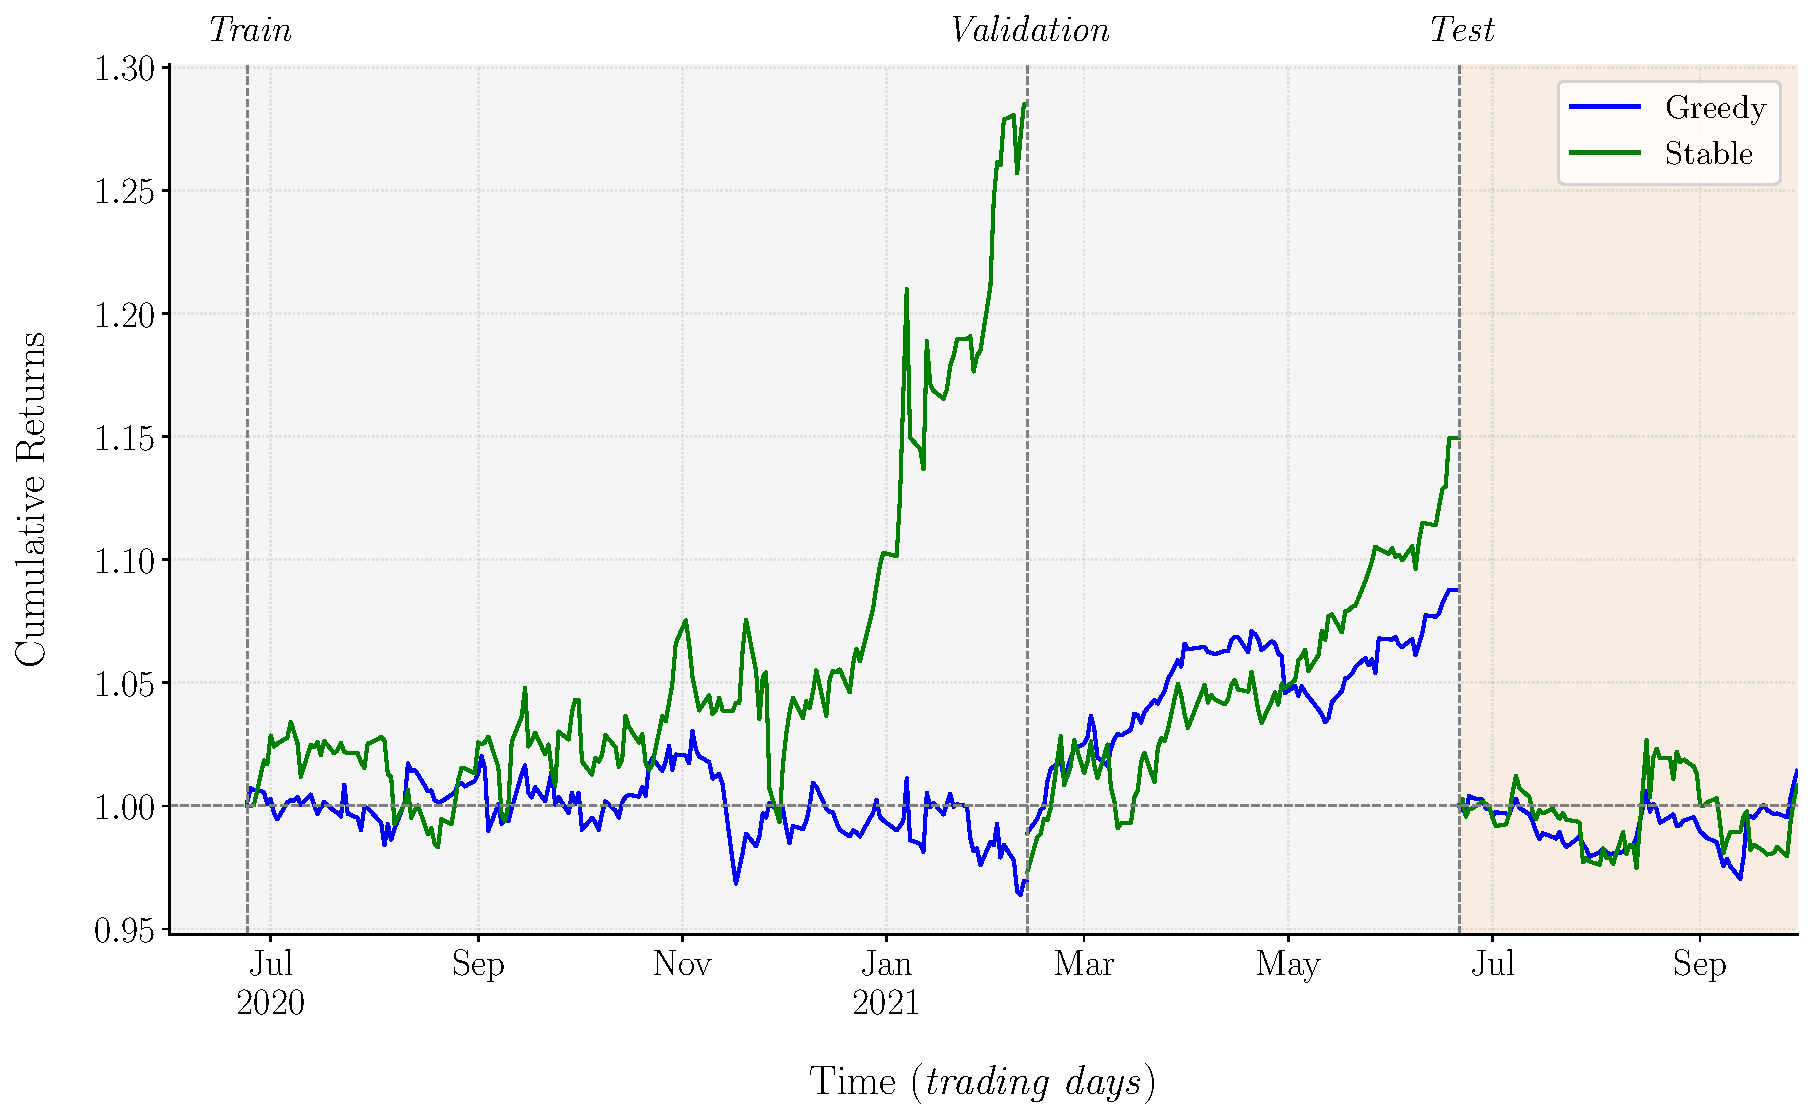
\includegraphics[scale=0.44]{fig_7a_KMeans_Portfolio.pdf}
\end{subfigure}

\vspace{0.75cm}

% Panel B: LLM
\begin{subfigure}{\textwidth}
\caption{Panel B: Cumulative Gross Returns of $\mathcal{P}_{\text{LLM}}$}
\centering
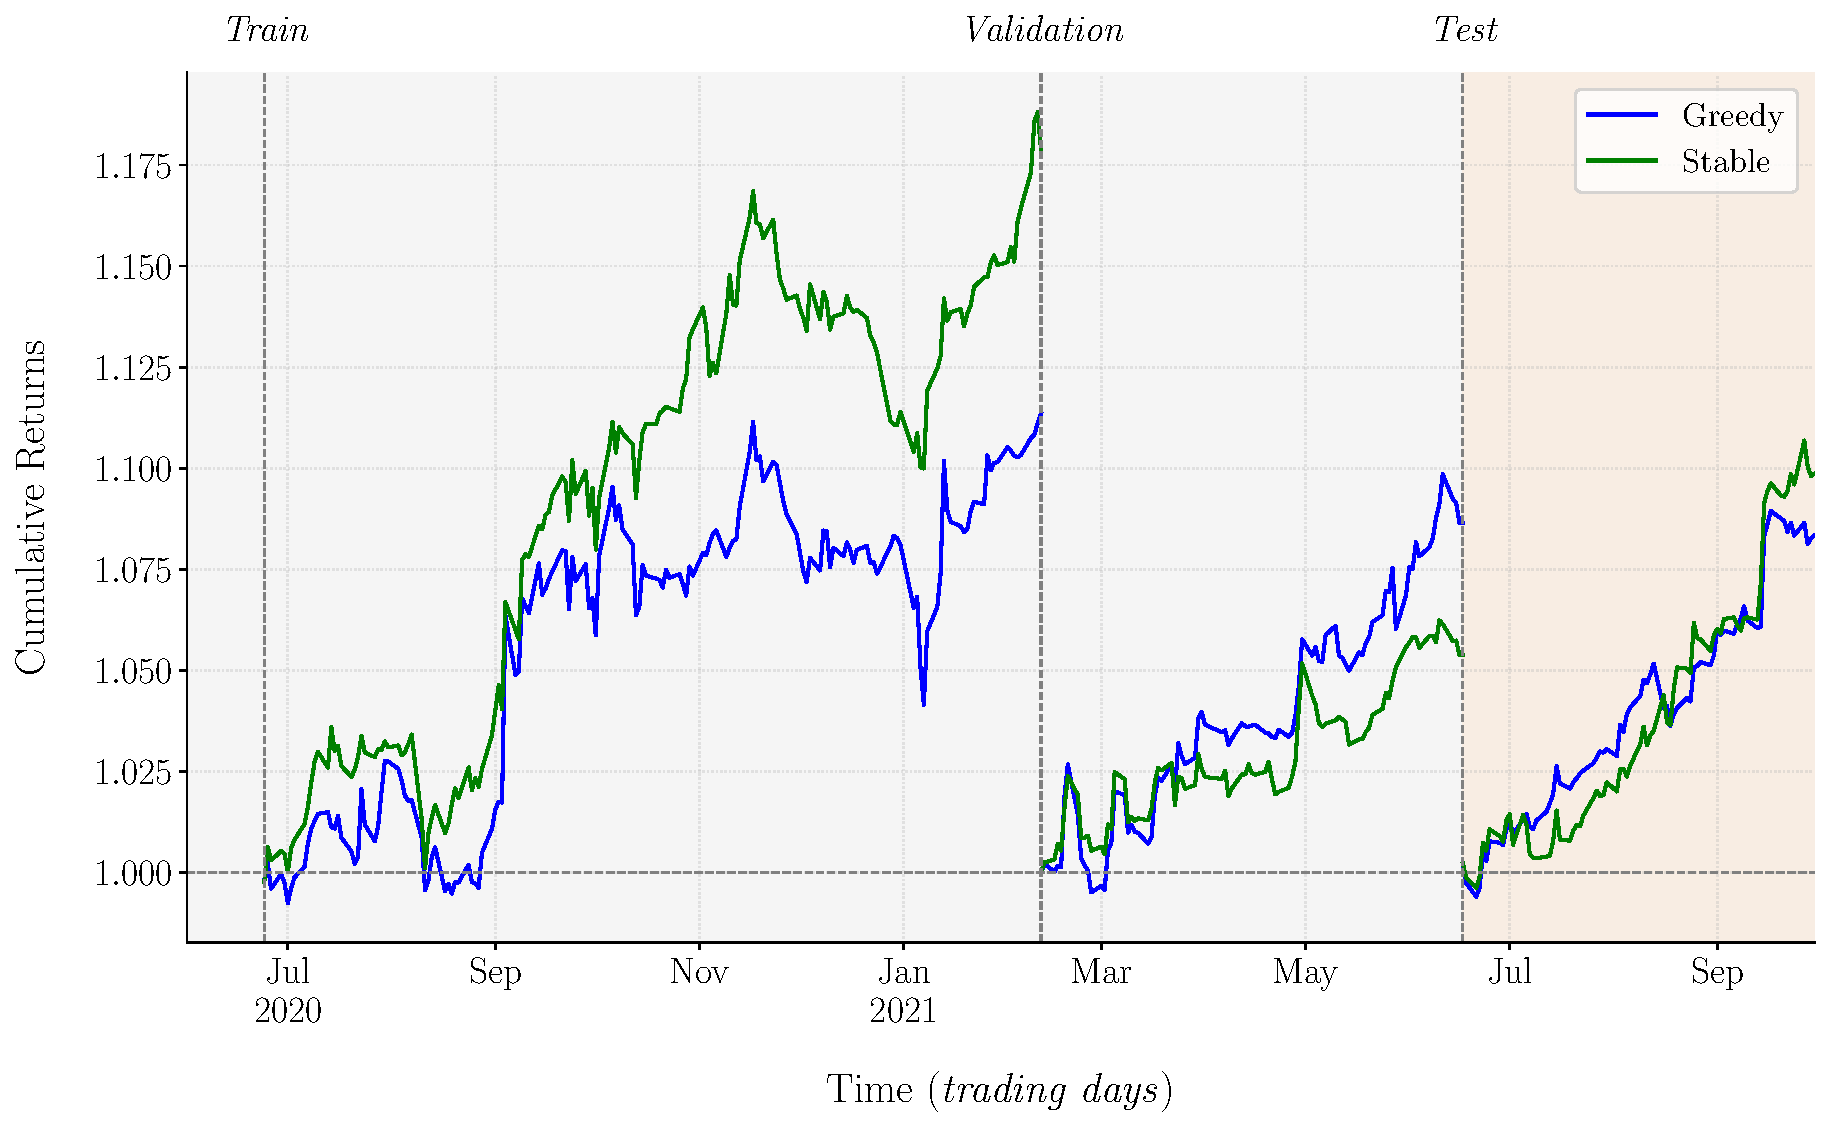
\includegraphics[scale=0.44]{fig_7b_LLAMA_Portfolio.pdf}
\end{subfigure}

\vspace{0.5cm}
\begin{minipage}{\textwidth}
\setlength{\parindent}{0pt}
{\footnotesize\textit{Note:} 
This figure presents the cumulative gross returns of trading strategies based on KMeans clustering (Panel A) and LLM clustering (Panel B) across different data splits. For both approaches, the holding period of the beta-neutral strategies is set to $L=4$ trading days. The number of traded clusters differs between approaches: $\theta=\integer{0.5k}=13$ for KMeans ($k^*=26$ clusters) and $\theta=\integer{0.5k}=10$ for LLM ($k=20$ clusters). The selection criteria for these parameters is based on maximizing the Sharpe Ratios of the train and validation samples. The Test split is higlhighted with a yellow background.
%
%The two approaches show markedly different out-of-sample performance. The embeddings-based KMeans clusters (Panel A) demonstrate poor out-of-sample performance, indicating a lack of robustness and failure to generalize effectively over time. In contrast, the LLM-based clustering approach (Panel B) exhibits strong out-of-sample performance, suggesting that the LLM-derived clusters effectively capture and predict market reactions to firm-specific economic shocks implied by news.
}
\end{minipage}
\end{figure}
%----------------------------------------------------

%%%%%%%%%%%%%%%%%%%  KMEANS %%%%%%%%%%%%%%%%%%%%%%%%%

\textbf{KMeans}. 
In panel A of \cref{tab:portfolio_statistics_gross_comparison} we show the portfolio statistics of the benchmark model.
As we can see, both algorithms work well on the data splits they were trained on: the Stable algorithm works well on both, training and validation data, while the Greedy algorithm does a good job only on validation data as expected. However, this doesn't say anything about any of these algorithms, as it is easy to make profitable trades \textit{in-sample}. 
%
The generalizability of the strategy is determined \textit{out-of-sample} in the test data. The empirical analysis reveals significant challenges in the strategy's ability to maintain consistent performance across different time periods. During the training and validation phases, the methodology shows promising results with annualized returns ranging from 26.6\% to 47.7\% and strong risk-adjusted performance metrics (Sharpe ratios between 2.0 and 3.2). However, this performance deteriorates substantially in the test period, where returns drop to modest levels (2.9\% to 4.9\% annually) with significantly lower Sharpe ratios (0.2 to 0.7), suggesting that the strategy's alpha-generating capability does not generalize well out of sample. The distributional properties of returns in the test period provide additional insights into the strategy's behavior under true out-of-sample conditions. The shift from negative to strongly positive skewness (1.85 to 2.46) coupled with high excess kurtosis (5.50 to 14.57) suggests that the strategy's return distribution has fundamentally changed, characterized by more frequent small losses offset by occasional large gains. This asymmetric return pattern, while potentially appealing from a risk preference perspective, differs markedly from the training period characteristics. The tail risk measures further illuminate the strategy's risk profile, with annualized 95\% VaR ranging from -7.8\% to -18.9\% and corresponding CVaR from -9.7\% to -26.8\% in the test period. These statistical properties, combined with the strong dependence on historical cluster-specific performance, indicate that the strategy fails to identify stable and generalizable trading signals, likely due to its reliance on firm and industry-specific clustering patterns that do not persist out of sample. As we can see in the plot, neither algorithm is able to generate a consistent profile of earnings, and the statistics confirm that profits are negligible, and would likely be eaten away by exogenous market frictions (e.g. trading costs).

%----------------------------------------------------
\inserthere{tab:portfolio_statistics_gross_comparison}

\begin{table}[H] 
\caption{Portfolio Statistics Comparison: KMeans vs LLM Clustering
% | Gross Returns
} 
\centering
\label{tab:portfolio_statistics_gross_comparison}

\renewcommand{\arraystretch}{1.1}
\newcolumntype{P}[1]{>{\centering\arraybackslash}p{#1}}

% Panel A: KMeans
\begin{subtable}{\textwidth}
\caption{Panel A: Statistics of $\mathcal{P}_{\text{KMeans}}$}
\centering
{\small
\begin{tabular}{
 P{1.28cm} P{0.9cm} P{0.9cm} P{0.9cm} P{0.9cm} P{0.9cm} P{0.9cm} 
 P{0.9cm} P{1cm} P{0.9cm} P{0.9cm} P{0.9cm} P{0.9cm}
}
\Xhline{2\arrayrulewidth}
\textbf{Split} & \textbf{Algo.} & \textbf{Cum. Ret.} & \textbf{Avg. Ret.} & \textbf{St. Dev.} & \textbf{Sharpe Ratio} & \textbf{Sortino Ratio} & \textbf{Max. DD} & \textbf{Calmar Ratio} & \textbf{Skew.} & \textbf{Exc. Kurt.} & \textbf{VaR 95\%} & \textbf{CVaR 95\%} \\
\Xhline{2\arrayrulewidth}
\multirow{2}{*}{All} & \textit{Greedy} & 1.070 & 5.3 & 9.7 & 0.5 & 0.6 & -6.9 & 0.8 & -0.45 & 4.04 & -13.7 & -22.9 \\
 & \textit{Stable} & 1.489 & 35.8 & 16.8 & 1.8 & 2.2 & -7.6 & 4.7 & 0.19 & 5.08 & -22.6 & -36.1 \\
\hline
\multirow{2}{*}{Train} & \textit{Greedy} & 0.959 & -6.2 & 11.7 & -0.5 & -0.5 & -6.9 & -0.9 & -0.52 & 2.72 & -18.3 & -28.5 \\
 & \textit{Stable} & 1.250 & 40.4 & 19.6 & 1.7 & 2.0 & -7.6 & 5.3 & -0.22 & 3.24 & -29.3 & -43.1 \\
\hline
\multirow{2}{*}{Validation} & \textit{Greedy} & 1.088 & 26.8 & 7.3 & 3.3 & 3.7 & -3.5 & 7.8 & -0.47 & 1.17 & -9.5 & -15.9 \\
 & \textit{Stable} & 1.149 & 47.6 & 13.3 & 2.9 & 3.5 & -3.6 & 13.1 & -0.19 & 1.76 & -18.3 & -28.1 \\
\hline
\multirow{2}{*}{Test} & \textit{Greedy} & 1.014 & 4.9 & 6.9 & 0.7 & 1.0 & -3.6 & 1.4 & 1.85 & 5.50 & -7.8 & -9.7 \\
 & \textit{Stable} & 1.008 & 2.9 & 14.3 & 0.2 & 0.3 & -4.6 & 0.6 & 2.46 & 14.57 & -18.9 & -26.8 \\
\Xhline{2\arrayrulewidth}
\end{tabular}
}
\end{subtable}

\vspace{0.5cm}

% Panel B: LLM
\begin{subtable}{\textwidth}
\caption{Panel B: Statistics of $\mathcal{P}_{\text{LLM}}$}
\centering
{\small
\begin{tabular}{
 P{1.28cm} P{0.9cm} P{0.9cm} P{0.9cm} P{0.9cm} P{0.9cm} P{0.9cm} 
 P{0.9cm} P{1cm} P{0.9cm} P{0.9cm} P{0.9cm} P{0.9cm}
}
\Xhline{2\arrayrulewidth}
\textbf{Split} & \textbf{Algo.} & \textbf{Cum. Ret.} & \textbf{Avg. Ret.} & \textbf{St. Dev.} & \textbf{Sharpe Ratio} & \textbf{Sortino Ratio} & \textbf{Max. DD} & \textbf{Calmar Ratio} & \textbf{Skew.} & \textbf{Exc. Kurt.} & \textbf{VaR 95\%} & \textbf{CVaR 95\%} \\
\Xhline{2\arrayrulewidth}
\multirow{2}{*}{All} & \textit{Greedy} & 1.310 & 23.1 & 9.6 & 2.2 & 2.9 & -6.3 & 3.7 & 1.47 & 9.93 & -13.6 & -18.9 \\
 & \textit{Stable} & 1.365 & 27.0 & 8.6 & 2.8 & 3.4 & -5.9 & 4.6 & 0.28 & 2.24 & -11.9 & -16.9 \\
\hline
\multirow{2}{*}{Train} & \textit{Greedy} & 1.112 & 17.6 & 11.4 & 1.4 & 1.9 & -6.3 & 2.8 & 1.65 & 9.00 & -15.7 & -21.0 \\
 & \textit{Stable} & 1.177 & 28.3 & 9.9 & 2.5 & 3.0 & -5.9 & 4.8 & 0.16 & 1.71 & -13.5 & -19.6 \\
\hline
\multirow{2}{*}{Validation} & \textit{Greedy} & 1.091 & 28.0 & 8.2 & 3.0 & 4.0 & -3.1 & 9.1 & 0.14 & 1.37 & -10.6 & -16.8 \\
 & \textit{Stable} & 1.048 & 14.2 & 7.0 & 1.9 & 2.1 & -1.9 & 7.4 & 0.25 & 1.37 & -11.1 & -14.7 \\
\hline
\multirow{2}{*}{Test} & \textit{Greedy} & 1.084 & 30.8 & 6.2 & 4.3 & 6.0 & -1.5 & 21.0 & 1.49 & 8.30 & -6.9 & -9.9 \\
 & \textit{Stable} & 1.100 & 37.2 & 7.1 & 4.4 & 7.2 & -1.1 & 34.5 & 0.84 & 1.95 & -9.5 & -11.3 \\
\Xhline{2\arrayrulewidth}
\end{tabular}
}
\end{subtable}

\vspace{0.5cm}
\begin{minipage}{\textwidth}
\setlength{\parindent}{0pt}
{\small\textit{Note:
Portfolio statistics of trading strategies based on clusters obtained from KMeans (Panel A) and LLM (Panel B) approaches.
The statistics provided include performance metrics (Cumulative Return, Average Return (\%)), risk measures (Standard Deviation (\%), Maximum Drawdown (\%), Value at Risk (\%), Conditional Value at Risk (\%)), risk-adjusted performance ratios (Sharpe Ratio, Sortino Ratio, Calmar Ratio), and return distribution characteristics (Skewness, Excess Kurtosis). These statistics are provided for both cluster-selection algorithms: Greedy and Stable.
Except for the Cumulative Return, all returns are annualized. The Sharpe Ratio is computed using the daily returns, assuming 252 trading days in a year. The Sortino Ratio is calculated using the daily downside returns. The Maximum Drawdown is the maximum loss from a peak to a trough. The Calmar Ratio is the ratio of the annualized return to the maximum drawdown. Skewness measures the asymmetry of the return distribution, while Kurtosis quantifies the tails' thickness. The Value at Risk (VaR) and Conditional Value at Risk (CVaR) are calculated at a 95\% confidence level.
The Greedy algorithm longs (shorts) clusters that maximize (minimize) the cluster-average-$SR$ in the validation sample subject to a positivity (negativity) constraint, while the Stable algorithm longs (shorts) clusters that minimize the rank difference between the training and validation rankings of the cluster-average-$SR$'s subject to a positivity (negativity) constraint, which is now imposed on both sample splits. In both algorithms, the cardinality of each leg is upper-bounded by a hyperparameter $\theta$.
The holding period of the beta-neutral positions is set to $L$ = 4 trading days for both approaches. The number of traded clusters is $\theta = 0.5k=13$ for KMeans ($k^*=26$ clusters) and $\theta = 0.5k=10$ for LLM ($k^*=20$ clusters). The selection criteria for these hyperparameters ($L,\theta$) is based on maximizing the Sharpe Ratios of the train and validation samples.
}}
\end{minipage}
\end{table}
%----------------------------------------------------


%%%%%%%%%%%%%%%%%%%%%% LLM %%%%%%%%%%%%%%%%%%%%%%%%%%%

\mx
\textbf{LLM}. 
%In panel B of \cref{tab:portfolio_statistics_gross_comparison} we show the portfolio statistics of the LLM-based strategy.
Panel B of \cref{tab:portfolio_statistics_gross_comparison} presents the performance metrics for our LLM-based approach.
As before, both algorithms perform really well on ``seen'' data. However, different from before, the \textit{Greedy} algorithm works well also on the Training Split (which it was not trained on). More importantly, both algorithms do a great job in the test data. As we can see, both are able to achieve a consistent profile of earnings through the split. 
%
The portfolio statistics 
%in Panel B of \cref{tab:portfolio_statistics_gross_comparison} 
reveal notable consistency in the strategy's performance across different time periods. During the training and validation phases, the methodology demonstrates solid performance with annualized returns ranging from 16.0\% to 28.3\% and Sharpe ratios between 1.4 and 2.9. This performance strengthens in the test period, where returns increase to 30.8\%-37.2\% annually with Sharpe ratios of 4.3-4.4, indicating that the strategy's alpha-generating capability successfully generalizes to out-of-sample conditions. The distributional properties of returns provide evidence for the strategy's robustness. 
%
The test period maintains positive skewness (0.84 to 1.49) and moderate to high excess kurtosis (1.95 to 8.30), indicating an asymmetric return pattern with more frequent small losses offset by larger gains. This return distribution is complemented by contained maximum drawdowns (1.1\% to 1.5\%) and strong Calmar ratios (21.0 to 34.5) in the test period. The tail risk measures further support the strategy's risk management properties, with annualized 95\% VaR ranging from -6.9\% to -9.5\%, and CVaR ranging from -9.9\% to -11.3\% in the test period. 
%
Taken together, the strategy's ability to sustain consistent out-of-sample performance metrics demonstrates that the LLM-based clustering approach identifies enduring trading signals that transcend specific market regimes.

%----------------------------------------------------

While our primary focus has been on developing a methodology to anticipate market reactions to news (i.e., identifying winners and losers to assess the predictive power of our LLM-based approach), we also analyze the trading intensity and implementation costs of the resulting strategies. The detailed examination in \ref{sec:A8} reveals that, under conservative transaction costs of 30 basis points per trade, the LLM-based approach maintains its superior performance relative to KMeans, though with attenuated profitability. Specifically, while KMeans strategies generate significant losses out-of-sample (-20.0\% to -23.6\% annually), our LLM-based approach achieves near-neutral to slightly positive net returns (-1.5\% to +3.1\%) in the test period, with notably lower risk metrics. These results underscore that while our methodology successfully captures predictable market reactions to news, practitioners implementing such strategies would benefit from incorporating transaction costs into their optimization framework.